\documentclass[12pt]{article}
\usepackage[margin=1in]{geometry}
\usepackage{setspace}
\onehalfspacing

\usepackage[T1]{fontenc}
\usepackage{lmodern}
\usepackage{microtype}
\usepackage{amsmath,amssymb,amsfonts}
\usepackage{booktabs}
\usepackage{tabularx}
\usepackage{graphicx}
\usepackage{caption}
\usepackage{subcaption}
\usepackage[authoryear,round]{natbib}
\usepackage{xcolor}
\usepackage{hyperref}
\hypersetup{
  colorlinks=true,
  linkcolor=blue!80!black,
  citecolor=blue!80!black,
  urlcolor=blue!80!black
}

\title{\textbf{Latent Trajectories of Cultural Taste During the Transition to College}}
\author{\textbf{Omar Lizardo} \\ Department of Sociology \\ University of California, Los Angeles}
\date{September 8, 2026}

\begin{document}

\maketitle

\begin{abstract}
Does higher education homogenize cultural tastes, or does it preserve and specialize pre-existing aesthetic boundaries? While cross-sectional research links scholastic capital to cultural omnivorousness, how individuals traverse distinct developmental pathways across specific activities during college remains underexplored. Using longitudinal panel data from the NetSense study, we investigate taste trajectories across two expressive cultural domains: leisure book reading (9 genres across six waves) and musical genre preferences (10 genres across six waves) ($N = 201$). We estimate multivariate binary latent class growth models in \texttt{flexmix} using natural cubic splines with endogenous multinomial concomitants. Across both spheres, a three-class specification provides optimal substantive parsimony, distinguishing omnivorous consumers, genre-selective specialists, and disengaged participants. Longitudinal analyses show that private cultural tastes divide into persistent, parallel developmental tracks with localized reallocations (such as surges in biography reading and country music adoption among omnivores), rather than pervasive collegiate homogenization or aesthetic boundary decay. Endogenous concomitants indicate that pre-collegiate academic capital universally predicts omnivorousness, whereas gender identity and academic major sort students into distinct subcultures. Finally, within-class growth models indicate that sociodemographics serve primarily as initial sorting gates into developmental pathways rather than moderating trajectory slopes within them.

\vspace{0.8em}
\noindent\textbf{Keywords:} Cultural Taste, Latent Class Growth Analysis, Cultural Omnivorousness, Higher Education, Emerging Adulthood, Finite Mixture Models
\end{abstract}

\newpage

\section{Introduction}

The evolution of cultural taste during emerging adulthood represents a central theoretical concern in the sociology of culture and higher education. The collegiate environment is frequently conceptualized as an incubator of aesthetic orientation, providing students with dense social networks, institutional opportunity structures, and exposure to diverse expressive forms. While cross-sectional scholarship has established durable connections between socioeconomic status, scholastic achievement, and cultural omnivorousness \citep{bourdieu1984distinction,peterson1996changing,lizardo2006cultural}, questions remain regarding how individuals traverse distinct developmental trajectories across specific cultural activities over the course of college.

Rather than aggregating participation into summary counts, examining separate binary items simultaneously allows researchers to observe whether taste change is uniform across an entire expressive sphere or driven by specific, institutionalized activities. Using longitudinal survey data from the NetSense study, this investigation models individual developmental pathways across two expressive domains: private leisure reading choices (tracked across 9 distinct book types from freshman through junior year) and musical genre preferences (tracked across 10 prominent musical genres from freshman through junior year). We implement a multivariate binary latent class growth model using natural cubic splines in the \texttt{flexmix} package \citep{grun2008flexmix} in \textsf{R} \citep{Rmanual}. This approach models individual-level trajectories for each item simultaneously while estimating endogenous multinomial concomitants to identify how sociodemographic background, academic achievement, and collegiate major structure latent class membership.

\section{Data and Measures}

\subsection{The NetSense Panel Study}

Empirical analyses use longitudinal survey microdata from the NetSense study, a multi-wave panel investigation tracking a cohort of undergraduate students matriculating at the University of Notre Dame in August 2011 \citep{striegel2013lessons}. NetSense recruited an initial cohort of incoming first-year students who were provided with sensor-enabled smartphones and surveyed repeatedly at each semester boundary across their undergraduate careers. Surveys captured detailed social networks, academic performance, sociodemographic backgrounds, and extensive inventories of expressive cultural practices.

Our analytical cohort comprises $N = 201$ undergraduate students with complete longitudinal reporting across all six consecutive semesters (Waves 1 through 6, Fall 2011 through Spring 2014), tracking participants continuously from freshman matriculation through junior year across both expressive cultural batteries.

\subsection{Expressive Cultural Batteries: Books and Music}

Across both expressive domains, cultural items are measured as binary indicators ($Y_{itj} \in \{0, 1\}$) reflecting semester-level participation or aesthetic preference. For leisure book reading, tracked across Waves 1 through 6, reading choices were measured by survey question Q47: ``\textit{During the past semester, what types of books did you read for pleasure or leisure (not for class assignments)?}'' Binary indicators were recorded across nine literary categories: mysteries and detective fiction; thrillers and suspense; romance; science fiction and fantasy; general and literary fiction; history, politics, and current affairs; biography and memoir; self-help and personal development; and general non-fiction and popular science.

For musical taste preferences, also tracked across Waves 1 through 6, preferences were measured by survey question Q44: ``\textit{Which of the following types of music do you like to listen to?}'' From the full 22-genre inventory administered in the survey, the 10 most prominent genres were selected for simultaneous multivariate trajectory modeling: classical music; dance music, electronica, and EDM; country and western; alternative and modern rock; classic rock and classic hits; Broadway and show tunes; pop and Top 40; jazz; folk and singer-songwriter; and rap and hip-hop.

\subsection{Baseline Sociodemographic and Scholastic Covariates}

To explain sorting into latent taste trajectories, we include nine baseline predictors measured at freshman matriculation, organized into four conceptual blocks. First, demographic identity includes gender identity (1 = Woman, 0 = Man), racial identification (1 = White, 0 = Students of Color), and religious preference (1 = Roman Catholic, 0 = Non-Catholic). Second, family socioeconomic status includes parental household pretax annual income, converted from 14 survey brackets to category midpoints in thousands of dollars (ranging from \$5,000 to \$300,000), alongside parental educational attainment, measured as the maximum years of schooling completed between mother and father (ranging from 10 to 18 years).

Third, pre-collegiate scholastic capital includes high school academic achievement (1 = Mostly A or A- grades, 0 = B+ or lower) and advanced degree aspirations (1 = Plans to pursue Master's, Ph.D., M.D., or J.D., 0 = Bachelor's degree only). Fourth, institutional and collegiate context encompasses declared undergraduate major (1 = Science, Technology, Engineering, or Mathematics, 0 = Arts, Humanities, or Business) and hometown urbanicity, measured on a 6-point scale ranging from rural farm to major metropolitan area. Missing values on baseline covariates (each under 6\% missingness) were handled via single predictive mean matching imputation in the \texttt{mice} package \citep{buuren2011mice} in \textsf{R} \citep{Rmanual}. Table~\ref{tab:descriptives} presents comprehensive descriptive statistics for all baseline covariates and cultural item batteries.

\begin{table}[htbp]
\centering
\footnotesize
\setlength{\tabcolsep}{1.8pt}
\renewcommand{\arraystretch}{0.92}
\caption{Descriptive Statistics for Baseline Covariates, Book Reading Types, and Music Genres ($N = 201$)}
\label{tab:descriptives}
\begin{tabular*}{\linewidth}{@{\extracolsep{\fill}}llcc@{}}
\toprule
Variable / Cultural Item & Operationalization & Mean / \% & SD / Wave Trend \\
\midrule
\multicolumn{4}{l}{\textbf{Panel A: Baseline Covariates ($N = 201$)}} \\
\quad Gender Identity & Woman (vs. Man) & 46.7\% & $n = 93$ \\
\quad Racial Identity & White (vs. Students of Color) & 67.8\% & $n = 135$ \\
\quad Religion & Roman Catholic (vs. Other) & 69.5\% & $n = 137$ \\
\quad Parental Income & Pretax bracket midpoint (\$1,000s) & \$121.4k & $\text{SD} = \$80.4\text{k}$ \\
\quad Parental Education & Highest parental schooling & 16.6 yrs & $\text{SD} = 1.8\text{ yrs}$ \\
\quad High School Grades & Mostly A or A- (vs. $\le$ B+) & 74.4\% & $n = 148$ \\
\quad Degree Aspirations & Post-BA (vs. BA only) & 91.5\% & $n = 182$ \\
\quad Academic Major & STEM Field (vs. Non-STEM) & 45.2\% & $n = 90$ \\
\quad Hometown Urbanicity & 6-point scale ($1 = \text{Rural}, 6 = \text{Metro}$) & 5.49 & $\text{SD} = 0.76$ \\
\addlinespace[3pt]
\multicolumn{4}{l}{\textbf{Panel B: Leisure Book Reading Types (Waves 1--6, $N = 201$)}} \\
\quad Science Fiction / Fantasy & Read for leisure & 56.1\% & W1: 58.8\% $\rightarrow$ W6: 52.6\% \\
\quad Mysteries / Detective & Read for leisure & 53.5\% & W1: 54.3\% $\rightarrow$ W6: 48.1\% \\
\quad General / Literary Fiction & Read for leisure & 53.4\% & W1: 56.8\% $\rightarrow$ W6: 51.9\% \\
\quad Thrillers / Suspense & Read for leisure & 42.8\% & W1: 42.7\% $\rightarrow$ W6: 43.7\% \\
\quad Biography / Memoir & Read for leisure & 35.3\% & W1: 45.7\% $\rightarrow$ W6: 31.1\% \\
\quad Self-Help / Development & Read for leisure & 34.5\% & W1: 38.2\% $\rightarrow$ W6: 40.7\% \\
\quad Romance & Read for leisure & 33.1\% & W1: 33.2\% $\rightarrow$ W6: 32.6\% \\
\quad General Non-Fiction / Science & Read for leisure & 24.2\% & W1: 31.2\% $\rightarrow$ W6: 20.0\% \\
\quad History / Politics / Current & Read for leisure & 15.9\% & W1: 18.1\% $\rightarrow$ W6: 17.0\% \\
\addlinespace[3pt]
\multicolumn{4}{l}{\textbf{Panel C: Musical Genre Preferences (Waves 1--6, $N = 201$)}} \\
\quad Classical Music & Likes to listen & 54.5\% & W1: 58.3\% $\rightarrow$ W6: 47.4\% \\
\quad Dance / Electronica / EDM & Likes to listen & 51.7\% & W1: 50.3\% $\rightarrow$ W6: 46.7\% \\
\quad Country / Western & Likes to listen & 50.7\% & W1: 44.2\% $\rightarrow$ W6: 53.3\% \\
\quad Alternative / Modern Rock & Likes to listen & 33.2\% & W1: 31.2\% $\rightarrow$ W6: 36.3\% \\
\quad Classic Rock & Likes to listen & 28.8\% & W1: 27.1\% $\rightarrow$ W6: 28.9\% \\
\quad Broadway / Show Tunes & Likes to listen & 19.5\% & W1: 19.1\% $\rightarrow$ W6: 17.0\% \\
\quad Pop / Top 40 & Likes to listen & 15.7\% & W1: 22.6\% $\rightarrow$ W6: 8.9\% \\
\quad Jazz & Likes to listen & 14.3\% & W1: 15.1\% $\rightarrow$ W6: 12.6\% \\
\quad Folk / Singer-Songwriter & Likes to listen & 13.1\% & W1: 11.1\% $\rightarrow$ W6: 12.6\% \\
\quad Rap / Hip-Hop & Likes to listen & 7.8\% & W1: 7.0\% $\rightarrow$ W6: 6.7\% \\
\bottomrule
\end{tabular*}
\begin{minipage}{\linewidth}
\vspace{4pt}
\footnotesize
\textit{Note:} Descriptive statistics computed across analytical cohort ($N = 201$ complete cases in Books and Music). Panel A shows baseline values before single stochastic imputation for missing items (each $< 6\%$ missingness). Panels B and C report pooled longitudinal prevalence across all six waves alongside initial Wave 1 and final Wave 6 empirical participation proportions.
\end{minipage}
\end{table}

\section{Methodological Framework}

\subsection{Multivariate Binary Mixture Formulation}

Let $i \in \{1, \dots, N\}$ index students observed across repeated survey waves $t \in \{1, \dots, T\}$. At each wave, students report binary participation ($Y_{itj} \in \{0, 1\}$) across a battery of $J$ distinct items ($J = 9$ for Book Types; $J = 10$ for Music Genres). In the multivariate binary mixture model, each item possesses its own distinct growth parameters within latent class $k \in \{1, \dots, K\}$.

Conditioned on membership in latent class $k$, the joint probability of observing an individual's vector of responses across all items and measurement waves is modeled as conditionally independent Bernoulli trials:
\begin{equation}
p(\mathbf{Y}_i \mid c_i = k) = \prod_{t=1}^{T} \prod_{j=1}^{J} \mu_{iktj}^{Y_{itj}} (1 - \mu_{iktj})^{1 - Y_{itj}}
\end{equation}
Repeated observations are grouped at the student level ensuring that latent class partitions reflect stable developmental archetypes across emerging adulthood.

\subsection{Harmonized Natural Spline Time Parameterization}

To achieve temporal flexibility without imposing the rigid symmetry or boundary instability of quadratic polynomials, the probability of endorsing item $j$ at time $t$ in class $k$ is parameterized via an inverse logit link using a natural cubic spline with two degrees of freedom, implemented via the \texttt{splines} package \citep{venables2002modern} in \textsf{R} \citep{Rmanual} (\texttt{splines::ns(time, df = 2)}):
\begin{equation}
\text{logit}(\mu_{iktj}) = \beta_{0kj} + \beta_{1kj} \text{ns}_1(t) + \beta_{2kj} \text{ns}_2(t)
\end{equation}
where $\text{Time}_{it} = \text{Wave}_{it} - 1$ centers time at collegiate matriculation ($t = 0$), and $\text{ns}_1(t)$ and $\text{ns}_2(t)$ represent orthogonalized natural spline basis functions with linear boundary constraints.

Across both expressive domains, students are observed over six consecutive semesters ($t \in \{0, \dots, 5\}$). Boundary knots are placed at $t = 0$ (Wave 1) and $t = 5$ (Wave 6), with an internal knot placed at the collegiate midpoint ($t = 2.5$, between sophomore fall and sophomore spring). This formulation captures developmental transitions across emerging adulthood while maintaining identical parametric complexity (three parameters per item per class) and enforcing linear boundary constraints at matriculation and junior year.

\subsection{Endogenous Multinomial Concomitant Models}

To avoid the classification error and attenuation inherent in two-step estimation, latent class membership probabilities $\pi_{ik} = P(c_i = k \mid \mathbf{X}_i)$ are estimated jointly with item trajectories through an endogenous multinomial logit model (\texttt{FLXPmultinom}):
\begin{equation}
\pi_{ik} = \frac{\exp(\mathbf{X}_i \boldsymbol{\gamma}_k)}{\sum_{l=1}^K \exp(\mathbf{X}_i \boldsymbol{\gamma}_l)}
\end{equation}
where $\boldsymbol{\gamma}_1 = \mathbf{0}$ sets Class 1 as the reference baseline. Across both expressive domains, the exact same battery of nine baseline predictors is included simultaneously: sociodemographic background (gender identity, racial identification, and religious affiliation); family socioeconomic status (parental household income and parental educational attainment); pre-collegiate scholastic capital (high school academic performance and advanced degree aspirations); and institutional and geographic context (declared STEM major and hometown urbanicity).

\section{Latent Class Selection Across Domains}

We evaluate candidate specifications from one through five latent classes ($K = 1 \dots 5$) across both expressive domains, following standard class enumeration protocols for latent growth mixture models \citep{nylund2007deciding}. Table~\ref{tab:selection} presents model fit statistics, stepwise Likelihood Ratio Tests (LRT), and student-level class distributions.

\begin{table}[htbp]
\centering
\footnotesize
\setlength{\tabcolsep}{3.5pt}
\caption{Model Fit Statistics and Class Proportions across Candidate Specifications ($K = 1 \dots 5$)}
\label{tab:selection}
\begin{tabular*}{\linewidth}{@{\extracolsep{\fill}}lccccccr@{}}
\toprule
Model & LogLik & Par & AIC & BIC & Stepwise $\chi^2$ ($df$) & $p$ & Class Proportions (\%) \\
\midrule
\multicolumn{8}{l}{\textbf{Panel A: Book Reading Types (9 Items, Waves 1--6, $N = 201$)}} \\
$K = 1$ & -5688.1 & 27 & 11430.2 & 11562.8 & --- & --- & 100\% \\
$K = 2$ & -5282.5 & 55 & 10675.0 & 10945.2 & 811.2 (28) & $< .001$ & 45.8\% / 54.2\% \\
$K = 3$ & -5015.5 & 83 & 10197.1 & 10604.9 & 533.9 (28) & $< .001$ & 29.9\% / 39.3\% / 30.8\% \\
$K = 4$ & -4849.1 & 111 & 9920.1 & 10465.5 & 333.0 (28) & $< .001$ & 21.4\% / 21.9\% / 29.9\% / 26.9\% \\
$K = 5$ & -4721.6 & 139 & 9721.3 & 10404.3 & 254.9 (28) & $< .001$ & 22.4\% / 16.4\% / 22.9\% / 11.9\% / 26.4\% \\
\addlinespace[3pt]
\multicolumn{8}{l}{\textbf{Panel B: Music Genre Preferences (10 Genres, Waves 1--6, $N = 201$)}} \\
$K = 1$ & -6262.8 & 30 & 12585.6 & 12733.0 & --- & --- & 100\% \\
$K = 2$ & -5783.4 & 61 & 11688.8 & 11988.6 & 958.8 (31) & $< .001$ & 48.3\% / 51.7\% \\
$K = 3$ & -5555.6 & 92 & 11295.1 & 11747.2 & 455.6 (31) & $< .001$ & 45.3\% / 23.4\% / 31.3\% \\
$K = 4$ & -5407.6 & 123 & 11061.1 & 11665.5 & 296.0 (31) & $< .001$ & 18.9\% / 22.4\% / 37.8\% / 20.9\% \\
$K = 5$ & -5276.7 & 154 & 10861.4 & 11618.2 & 261.8 (31) & $< .001$ & 8.5\% / 22.4\% / 16.9\% / 30.3\% / 21.9\% \\
\bottomrule
\end{tabular*}
\begin{minipage}{\linewidth}
\vspace{4pt}
\footnotesize
\textit{Note:} Models estimated in \texttt{flexmix} using natural cubic splines with 2 degrees of freedom (\texttt{splines::ns(time, df = 2)}). LogLik = maximized log-likelihood; Par = number of estimated free parameters; AIC = Akaike Information Criterion; BIC = Bayesian Information Criterion; Stepwise $\chi^2$ evaluates improvement over $K - 1$ specification.
\end{minipage}
\end{table}

Across both expressive domains, moving from a single homogeneous growth curve ($K = 1$) to a multi-class mixture produces marked improvements in predictive log-likelihood. In both leisure reading and music preferences, the three-class specification captures the primary structural elbow: moving from two to three classes yields large reductions in BIC \citep{raftery1995bayesian} ($\Delta\text{BIC} = -340.3$ in Books; $\Delta\text{BIC} = -241.4$ in Music; $p < 0.001$), generating well-populated, substantively cohesive groups of roughly equal size ($25\%$ to $45\%$). Substantively, $K = 3$ is optimal: it cleanly separates specialized cultural omnivores, focused genre specialists, and disengaged readers and listeners. Beyond three classes, solutions fragment existing classes into redundant sub-clusters. Consequently, $K = 3$ is selected as the primary substantive specification across both domains.

\section{Item-Specific Trajectory Profiles}

\subsection{Leisure Book Reading (9 Items)}

Figure~\ref{fig:books} illustrates the model-implied reading trajectories across all nine book categories for each of the three latent classes over all six collegiate semesters. Lines trace continuous natural cubic spline curves, while discrete geometric markers designate empirical survey wave observations. All trajectory profiles and small-multiple panels were visualized using the \texttt{ggplot2} package \citep{wickham2016ggplot2} in \textsf{R} \citep{Rmanual}.

\begin{figure}[htbp]
\centering
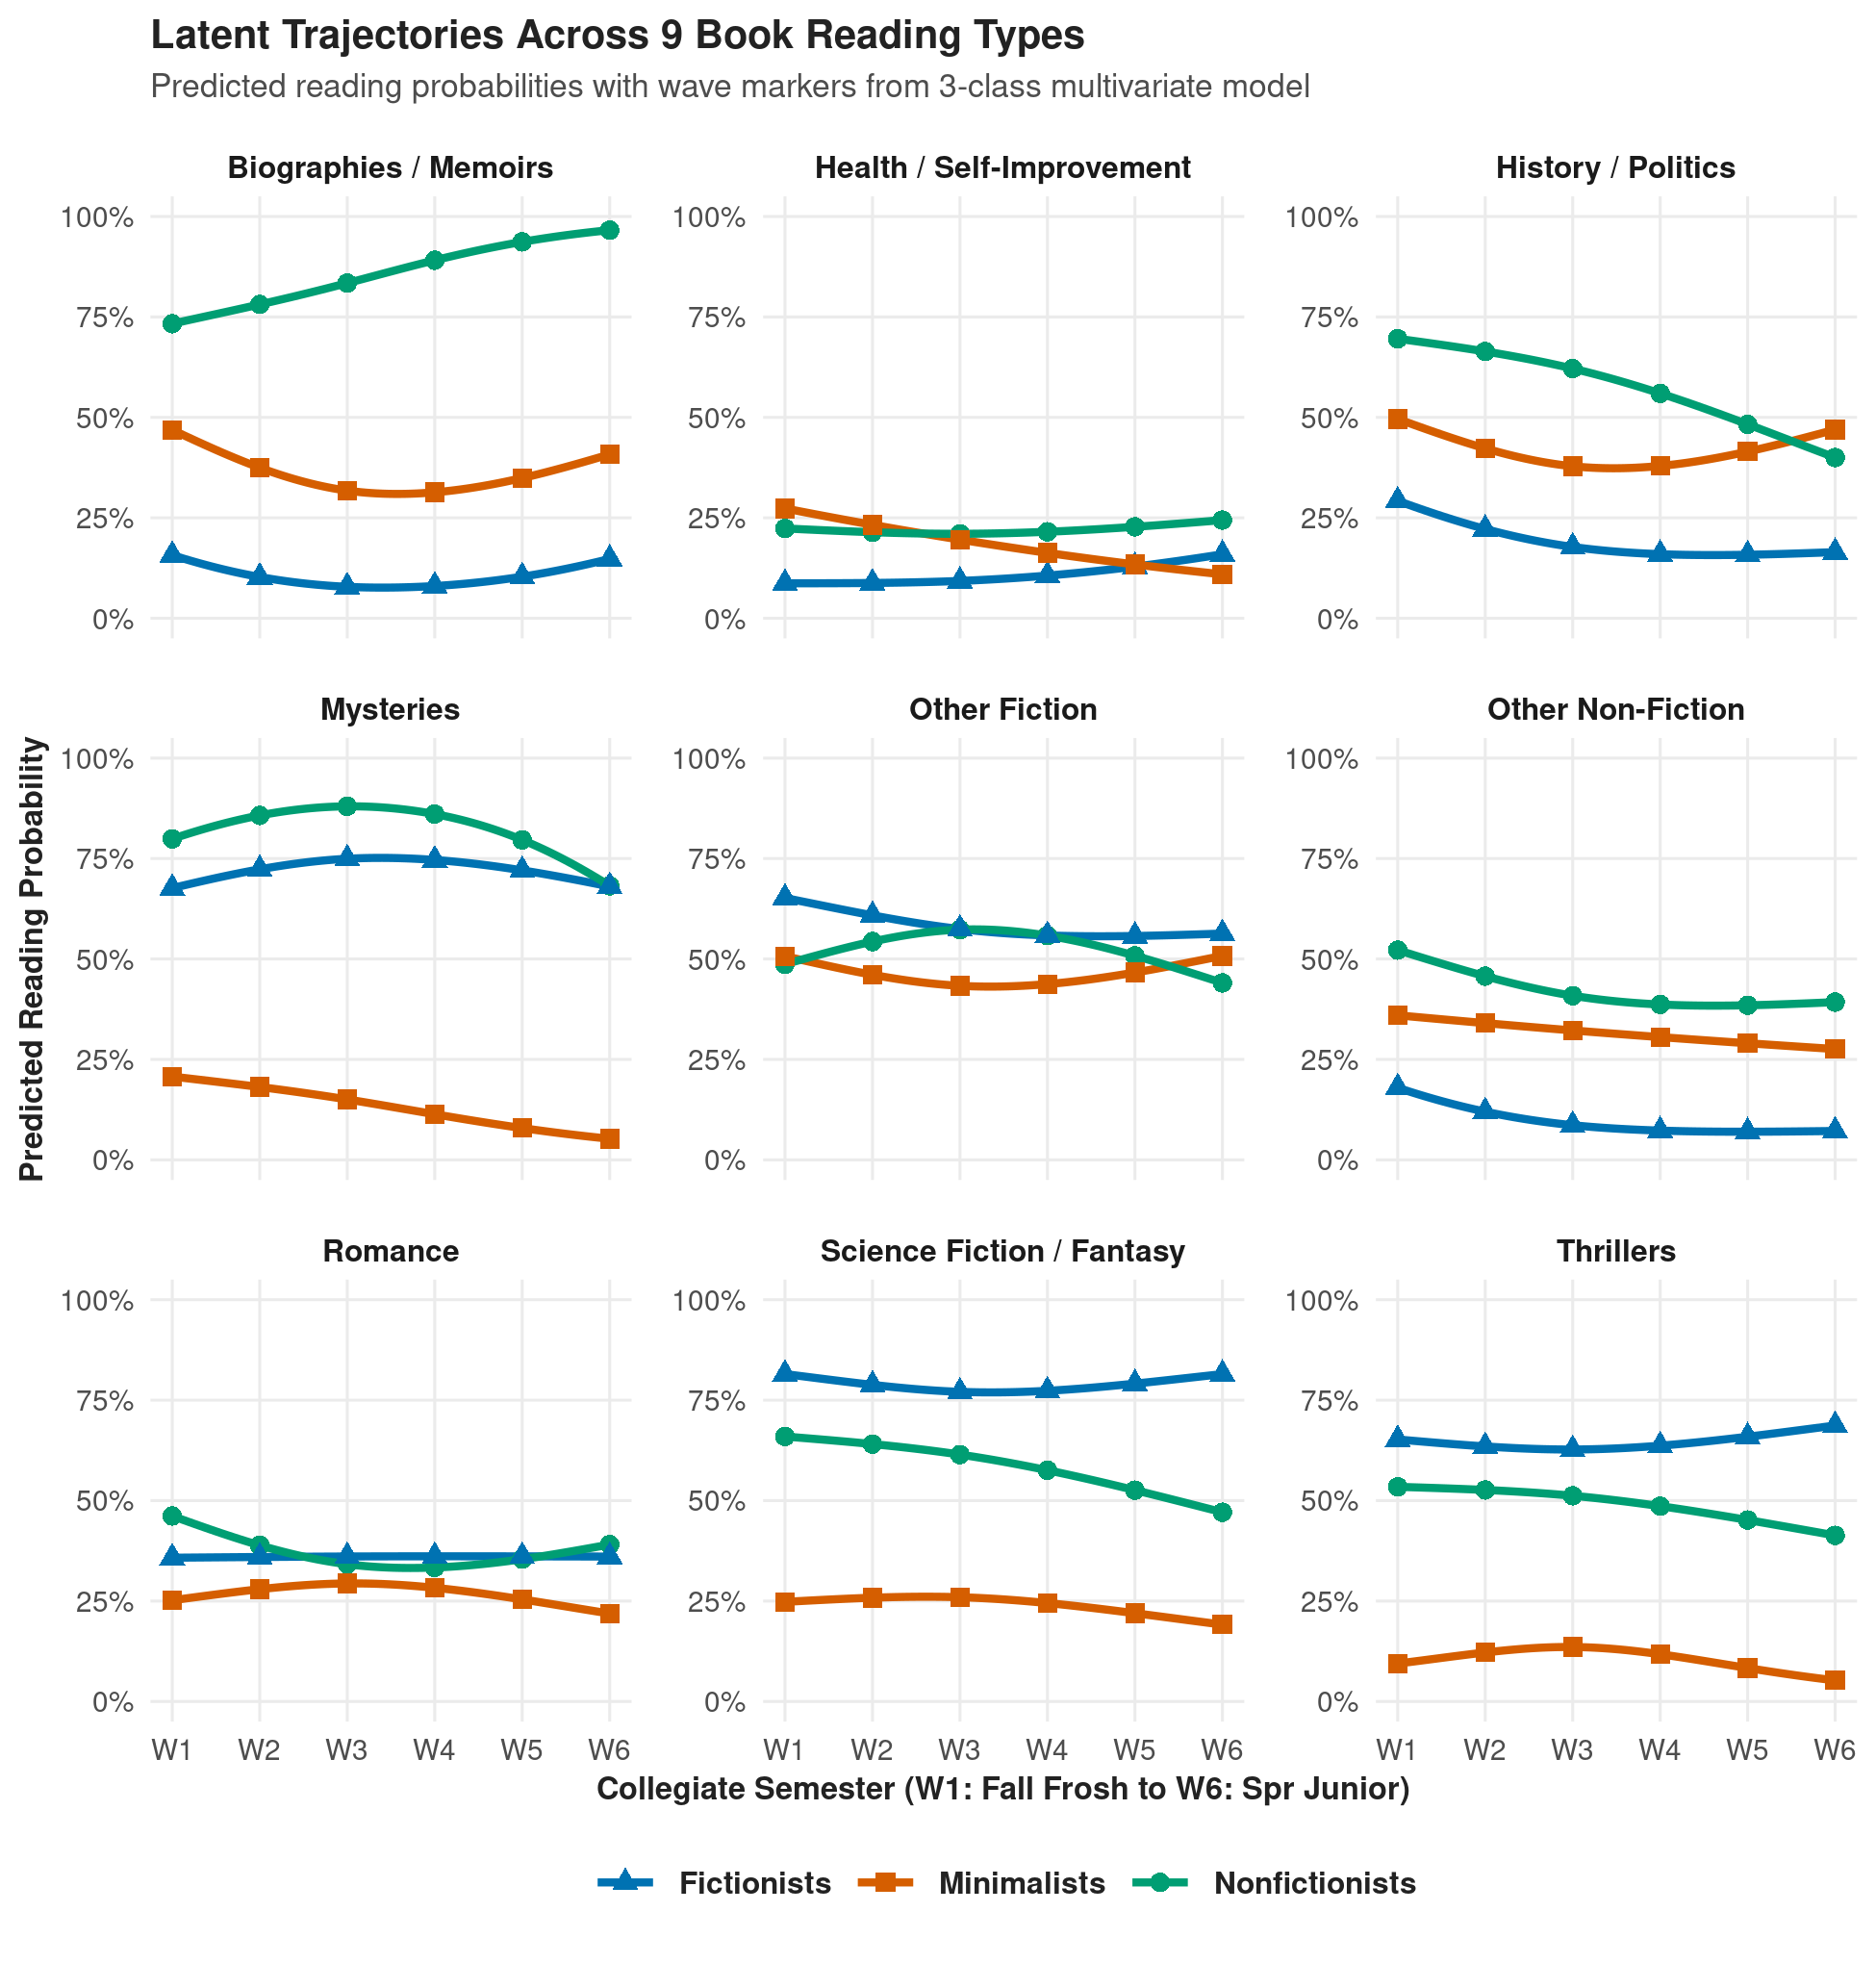
\includegraphics[width=\linewidth]{Plots/fig1_books_9_items_by_class.png}
\caption{Latent trajectories across 9 Book Reading Types from the 3-class multivariate binary model (Waves 1 to 6). Circles and green curves indicate Class 1 (``Nonfictionists''), triangles and blue curves indicate Class 2 (``Fictionists''), and squares and orange curves indicate Class 3 (``Minimalists'').}
\label{fig:books}
\end{figure}

The item-specific reading trajectories show that collegiate reading is structured by distinct aesthetic genre specializations rather than an undifferentiated continuum of reading volume. The first class, ``Class 1: Nonfictionists'' ($n = 60$, 29.9\%), exhibits an analytical, non-fiction reading profile: its members lead the student body in reading history and politics (69.6\%), biographies and memoirs (73.3\%), and general non-fiction (52.2\%), while reading little genre fiction. Over the course of college, Nonfictionists reallocate their leisure reading: reading of dense historical and political volumes decreases by 29.6 percentage points, accompanied by a surge in personal biographies and memoirs (rising from 73.3\% to 96.6\%, a +23.3 percentage point increase). The second group, ``Class 2: Fictionists'' ($n = 79$, 39.3\%), reads narrative genre fiction at elevated rates, maintaining high engagement with science fiction and fantasy (81.5\%), mysteries (67.6\%), thrillers (65.2\%), and general fiction (65.2\%), while reporting low interest in history and politics (29.2\%) and biographies (15.7\%). The third group, ``Class 3: Minimalists'' ($n = 62$, 30.8\%), exhibits consistently lower reading engagement across nearly all categories (thrillers 9.4\%, mysteries 20.7\%, science fiction 24.8\%). Reading trajectories remain remarkably stable across all six semesters, showing that literary orientations are established early and persist throughout college.

\subsection{Musical Taste Preferences (Top 10 Genres)}

Figure~\ref{fig:music} illustrates the model-implied preference trajectories across the top 10 musical genres for each of the three latent classes over all six collegiate semesters.

\begin{figure}[htbp]
\centering
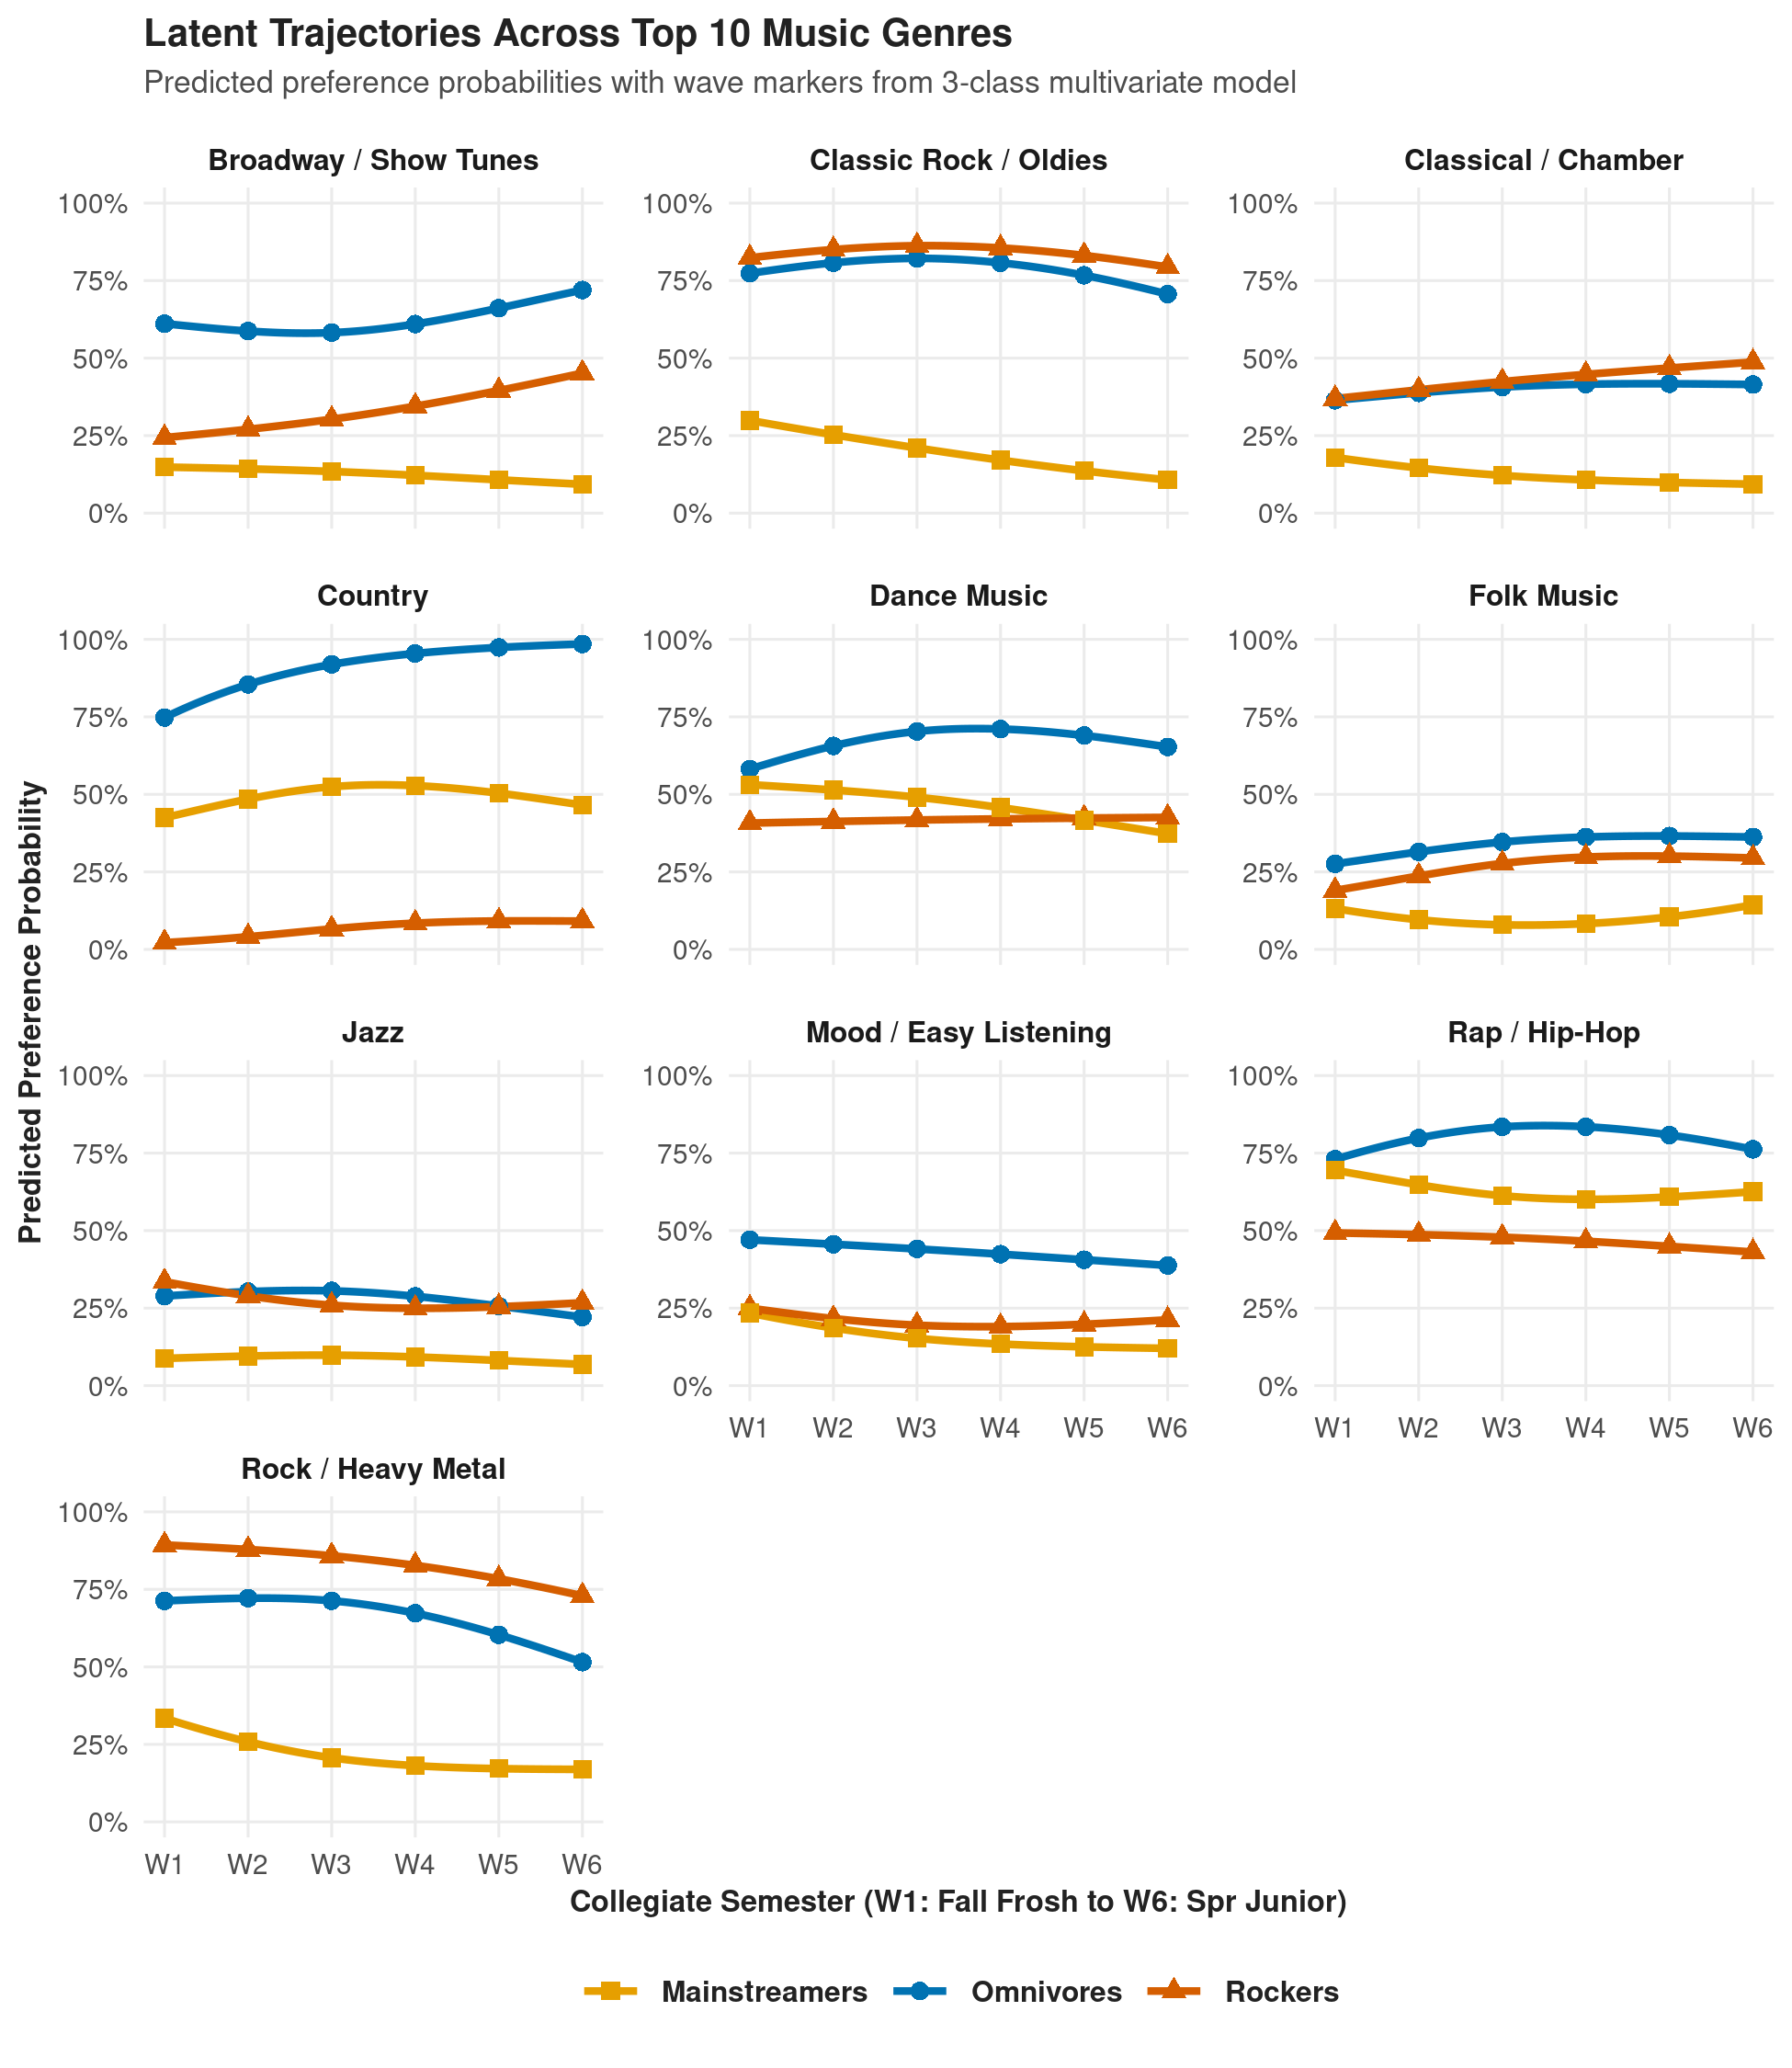
\includegraphics[width=\linewidth]{Plots/fig2_music_10_genres_by_class.png}
\caption{Latent trajectories across the Top 10 Music Genres from the 3-class multivariate binary model (Waves 1 to 6). Circles and blue curves denote Class 1 (``Omnivores''), triangles and red curves denote Class 2 (``Rockers''), and squares and orange curves denote Class 3 (``Mainstreamers'').}
\label{fig:music}
\end{figure}

Examining the item-level music trajectories shows how genre boundaries define distinct student taste cultures. The first class, ``Class 1: Omnivores'' ($n = 62$, 30.8\%), maintains high preference probabilities across all 10 genres simultaneously, embracing Broadway show tunes (61.1\%), classical music (36.4\%), folk (27.6\%), and country (74.8\%) alongside contemporary rap (73.0\%) and classic rock (77.3\%). Country music expands to near-universal adoption among Omnivores over time (+23.7 percentage points). The second group, ``Class 2: Rockers'' ($n = 51$, 25.4\%), exhibits a focused genre-selective profile: its members report near-universal preference for rock and heavy metal (89.3\%) and classic rock (82.4\%), but actively reject country music (2.2\%) and show low interest in folk and Broadway. The third group, ``Class 3: Mainstreamers'' ($n = 88$, 43.8\%), represents the commercial mainstream: they listen actively to rap/hip-hop (69.4\%), dance music (53.1\%), and country (42.5\%), but report low preference for highbrow classical (17.9\%), jazz (8.8\%), or folk music (13.2\%). Across all three classes, musical preferences remain exceptionally stable across all six semesters, even as rock and heavy metal displays a modest cross-class decline of 16 to 20 percentage points.

\subsection{Net Trajectory Shifts Within Latent Classes}

To evaluate how participation changes across the entire collegiate life course within each latent class, Figure~\ref{fig:shifts} displays the net percentage point shift ($\Delta = P(W_6) - P(W_1)$) for every cultural item across all three latent classes.

\begin{figure}[htbp]
\centering
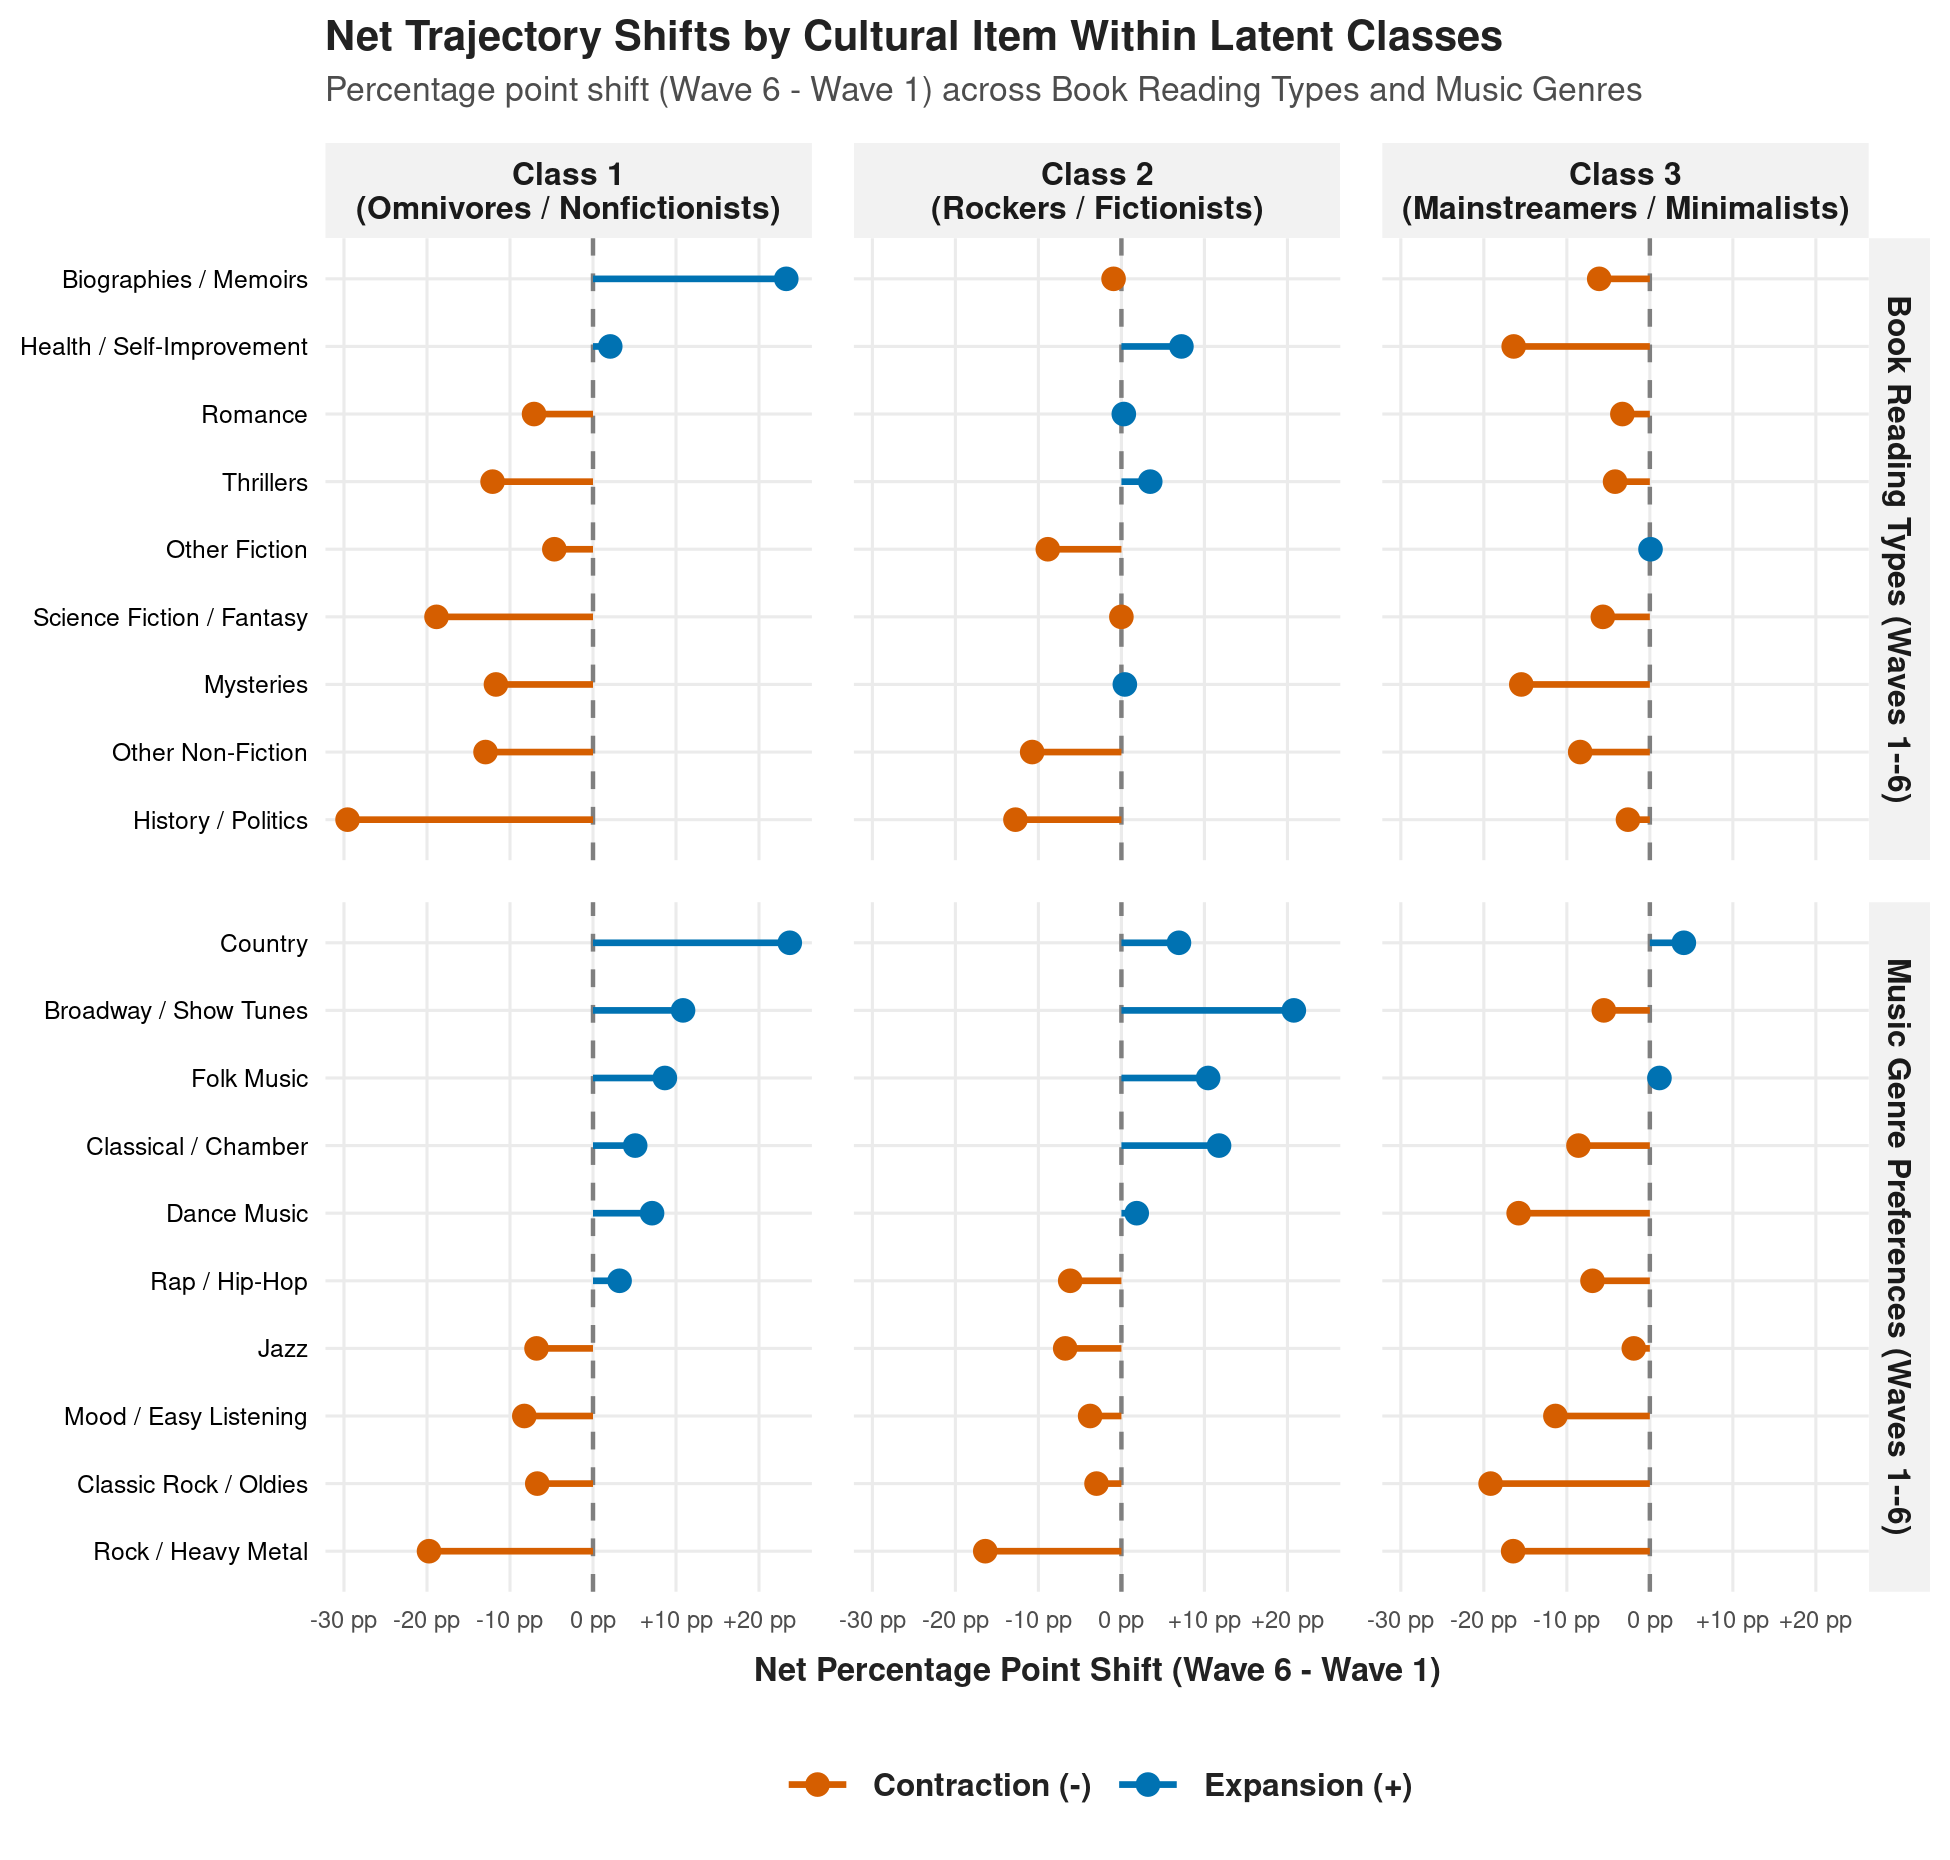
\includegraphics[width=\linewidth]{Plots/fig3_activity_time_trend_shifts.png}
\caption{Net trajectory shifts by cultural item within latent classes. Markers and connecting segments indicate the net percentage point shift ($\Delta = P(W_6) - P(W_1)$) from baseline matriculation to junior spring across Book Reading Types and Music Genres. Blue markers denote positive expansion; orange markers denote contraction.}
\label{fig:shifts}
\end{figure}

Examining net trajectory shifts reveals that collegiate cultural change is characterized by targeted reallocation within existing repertoires rather than wholesale aesthetic drift. Among Class 1 Nonfictionists in leisure reading, students substantially expand personal biography and memoir reading (+23.3 percentage points) while pruning dense historical and political reading (-11.7 to -18.9 percentage points). In contrast, Class 2 Fictionists maintain stable or slightly expanding reading rates across thrillers (+3.5 pp), mysteries (+0.4 pp), and sci-fi/fantasy (+0.3 pp), while Class 3 Minimalists exhibit contractions across every single book category (falling by up to -15.5 percentage points). In musical taste, Class 1 Omnivores uniquely expand country music adoption (+23.7 percentage points) alongside modest expansions in dance music (+3.6 pp) and classical music (+1.3 pp). In contrast, Class 2 Rockers actively contract their musical footprint across mainstream genres (rap falling by -16.2 pp and pop by -13.8 pp), while Class 3 Mainstreamers concentrate strictly on commercial hits, contracting highbrow jazz (-7.2 pp) and folk (-4.8 pp). These net shifts show that latent classes function as distinct developmental environments where students selectively reinforce specific aesthetic boundaries over time.

\section{Predicting Trajectory Class Membership}

\subsection{Predictive Power of Theoretical Variable Blocks}

To evaluate the overall contribution of competing theoretical explanations in structuring latent class assignment, Table~\ref{tab:blocks} presents Likelihood Ratio Tests (LRT $\chi^2$) and Wald $\chi^2$ statistics for each variable block evaluated against an empty baseline model.

\begin{table}[htbp]
\centering
\small
\setlength{\tabcolsep}{4.5pt}
\caption{Model Fit and Predictive Power of Theoretical Variable Blocks across Expressive Domains ($N = 201$)}
\label{tab:blocks}
\begin{tabular*}{\linewidth}{@{\extracolsep{\fill}}lcccccc@{}}
\toprule
Predictor Specification & Wald $\chi^2$ & LRT $\chi^2$ & $df$ & $p$ & AIC & BIC \\
\midrule
\multicolumn{7}{l}{\textbf{Panel A: Book Reading Types (9 Items, $N = 201$)}} \\
\quad Block 1: Demographic Identity & 94.64 & 94.64 & 6 & $< .001$ & 360.3 & 386.7 \\
\quad Block 2: Family SES & 0.89 & 0.89 & 4 & 0.926 & 450.0 & 469.9 \\
\quad Block 3: Scholastic Capital & 15.79 & 5.79 & 4 & 0.215 & 445.1 & 465.0 \\
\quad Block 4: Collegiate Context & 11.43 & 11.43 & 4 & 0.022 & 439.5 & 459.3 \\
\quad Combined Sociodemographics (Blocks 1+2) & 99.69 & 99.69 & 10 & $< .001$ & 363.2 & 402.9 \\
\quad Full Multivariable Model & 110.36 & 110.36 & 18 & $< .001$ & 368.6 & 434.6 \\
\addlinespace[3pt]
\multicolumn{7}{l}{\textbf{Panel B: Music Genre Preferences (10 Genres, $N = 201$)}} \\
\quad Block 1: Demographic Identity & 30.62 & 30.62 & 6 & $< .001$ & 415.8 & 442.2 \\
\quad Block 2: Family SES & 3.70 & 3.70 & 4 & 0.448 & 438.7 & 458.5 \\
\quad Block 3: Scholastic Capital & 19.72 & 19.72 & 4 & $< .001$ & 422.7 & 442.5 \\
\quad Block 4: Collegiate Context & 13.92 & 13.92 & 4 & 0.008 & 428.5 & 448.3 \\
\quad Combined Sociodemographics (Blocks 1+2) & 33.53 & 33.53 & 10 & $< .001$ & 420.8 & 460.5 \\
\quad Full Multivariable Model & 60.32 & 60.32 & 18 & $< .001$ & 410.1 & 476.1 \\
\bottomrule
\end{tabular*}
\begin{minipage}{\linewidth}
\vspace{4pt}
\footnotesize
\textit{Note:} LRT = Likelihood Ratio Test $\chi^2$ evaluated against the null (empty concomitant) baseline model within each domain. Block 1 includes Gender Identity, Racial Identity, and Religion; Block 2 includes Parental Household Income and Parental Education; Block 3 includes High School GPA and Advanced Degree Aspirations; Block 4 includes Academic Major (STEM) and Hometown Urbanicity.
\end{minipage}
\end{table}

The block tests provide compelling evidence regarding the social stratification of cultural trajectories. Demographic identity (Gender, Race, and Religion) significantly predicts class sorting across both domains: leisure reading ($\chi^2 = 94.64, df = 6, p < 0.001$) and music preferences ($\chi^2 = 30.62, df = 6, p < 0.001$). Pre-collegiate scholastic capital (GPA and degree aspirations) is highly significant in music ($\chi^2 = 19.72, df = 4, p < 0.001$), lowering AIC from 438.7 to 422.7. Collegiate context (STEM major and hometown urbanicity) significantly predicts class membership in both books ($\chi^2 = 11.43, df = 4, p = 0.022$) and music ($\chi^2 = 13.92, df = 4, p = 0.008$). In contrast, family socioeconomic status (parental income and education) is completely non-significant across both domains ($\chi^2 = 0.89, p = 0.926$ in books; $\chi^2 = 3.70, p = 0.448$ in music). When all blocks are combined, the full multivariable models achieve decisive statistical significance ($p < 0.001$ in both books and music).

\subsection{Model-Implied Marginal Class Probabilities}

While Table~\ref{tab:blocks} evaluates the overall predictive power of theoretical variable blocks, interpreting individual coefficients from multinomial logit models is often complicated by arbitrary reference baselines and non-linear log-odds metrics. Table~\ref{tab:app_coefs} in the Appendix reports the complete multivariable parameter estimates and odds ratios for all nine covariates across both domains. Following recent methodological practice in latent growth mixture analysis, we translate these multivariable model parameters into model-implied marginal predicted class probabilities with 95\% simulation confidence intervals, holding other background covariates constant at sample means and reference categories. Figure~\ref{fig:marginal} illustrates these marginal class probabilities across the statistically significant predictor blocks identified in Table~\ref{tab:blocks}.

\begin{figure}[htbp]
\centering
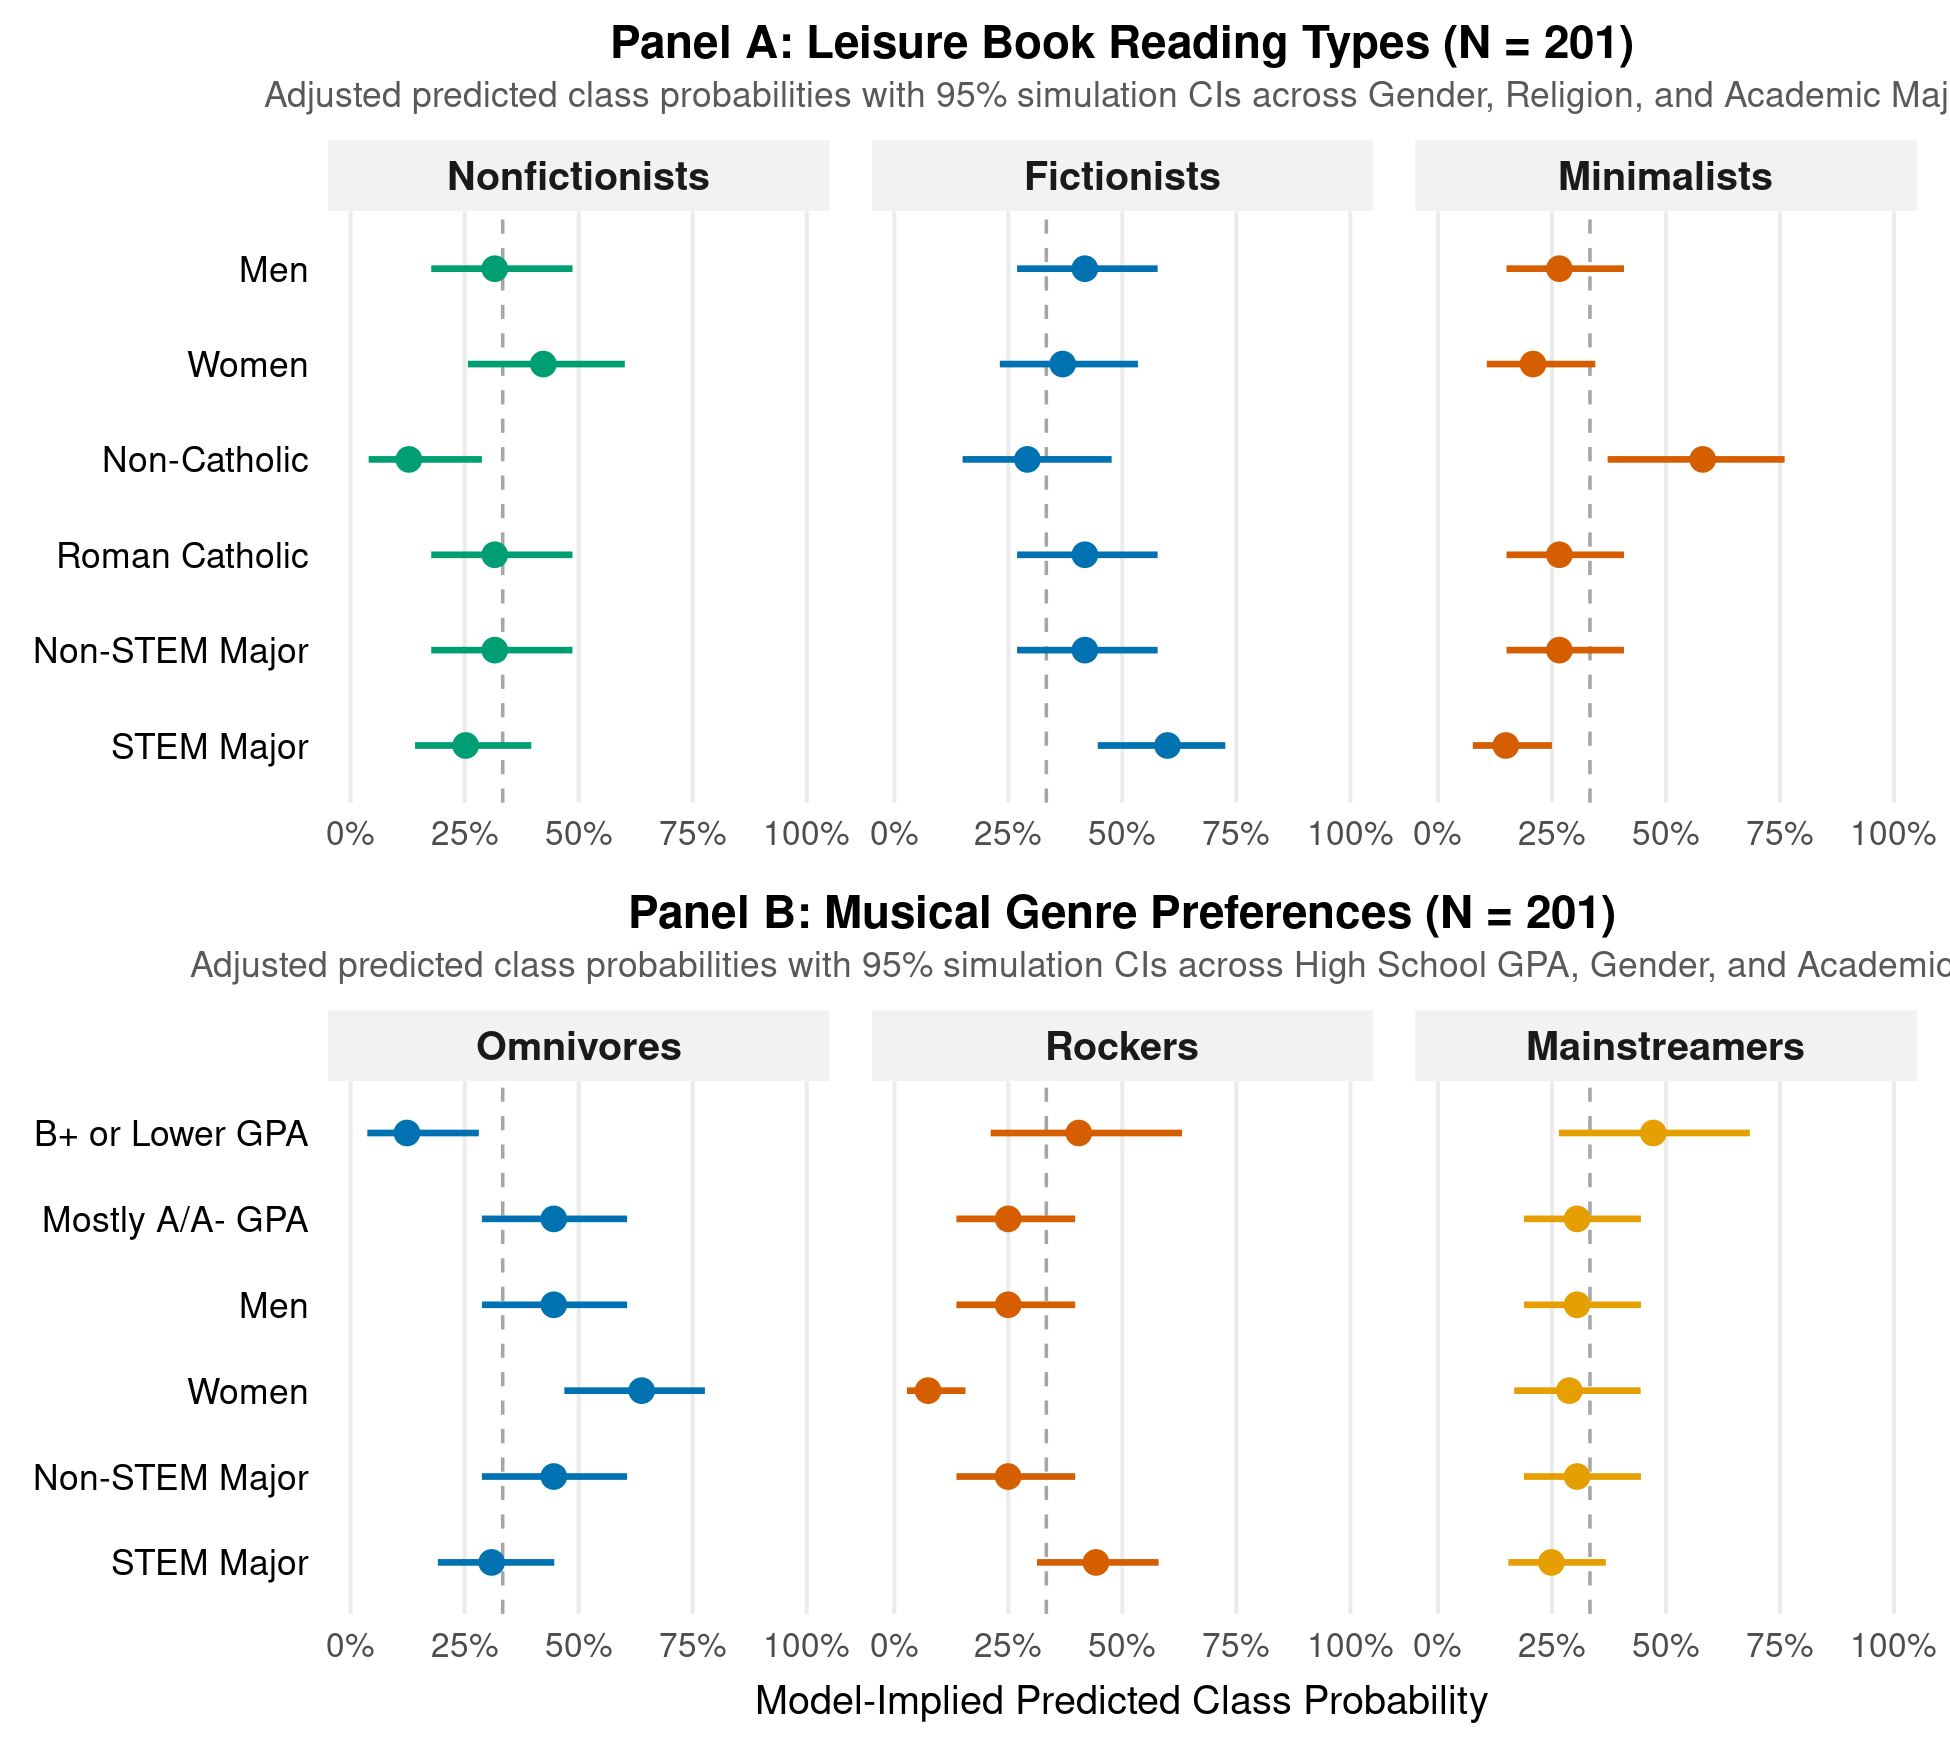
\includegraphics[width=\linewidth,height=0.65\textheight,keepaspectratio]{Plots/fig4_marginal_effects_books_music.png}
\caption{Model-implied marginal predicted trajectory class probabilities with 95\% simulation confidence intervals across statistically significant predictor blocks from Table~\ref{tab:blocks}. Panel A displays predicted probabilities for Leisure Book Reading Types across Gender Identity, Religion, and Undergraduate Major. Panel B displays predicted probabilities for Musical Genre Preferences across High School Academic Grades, Gender Identity, and Undergraduate Major. Dashed vertical reference lines indicate the equal random allocation baseline ($33.3\%$).}
\label{fig:marginal}
\end{figure}

In Panel A, Leisure Book Reading Types reveals that genre specializations are sharply divided by religious affiliation, gender identity, and undergraduate field of study. Religious identity produces pronounced sorting into reading styles: students identifying as Roman Catholic have a 31.6\% probability of belonging to Class 1 Nonfictionists and a 41.8\% probability of Class 2 Fictionists, with only a 26.6\% probability of sorting into Minimalist reading. Conversely, non-Catholic students are predominantly channeled into Class 3 Minimalist reading (58.1\%, 95\% CI: [37.2\%, 76.0\%]). Collegiate major also sorts students into distinct literary spheres: declared STEM majors exhibit a 59.9\% probability of belonging to Class 2 Fictionists (specializing in science fiction, fantasy, and thrillers) compared to 41.8\% among non-STEM students, alongside lower disengagement (14.9\% vs. 26.6\% for Minimalists).

In Panel B, Musical Genre Preferences illustrates the strong sorting power of pre-collegiate scholastic capital alongside gender identity and academic context. Earning mostly A/A- grades in high school serves as a primary sorting gateway into musical omnivorousness: high-achieving students have a 44.5\% probability of entering Class 1 Omnivores, compared to only 12.3\% (95\% CI: [3.7\%, 28.1\%]) among students with B+ or lower grades. Students entering with lower high school performance sort heavily into Class 3 Mainstreamers (47.2\%) and Class 2 Rockers (40.5\%). Gender identity sharply differentiates the rock subculture: men have a 25.0\% probability of sorting into Class 2 Rockers, whereas women have only a 7.4\% probability (95\% CI: [2.8\%, 15.6\%]), concentrating instead in Class 1 Omnivores (63.8\%). Finally, undergraduate major reinforces these aesthetic boundaries: declared STEM majors are significantly more likely to enter the Rocker pathway (44.2\%, 95\% CI: [31.3\%, 58.0\%]) than non-STEM majors (25.0\%), showing that collegiate fields of study cultivate distinct musical taste cultures.

Across both domains, parental socioeconomic status (income and parental education) displays negligible direct sorting power once prior academic achievement and demographic characteristics are controlled. Crucially, demographic characteristics operate almost exclusively as between-class sorting gates (the extensive margin) rather than within-class slope modifiers (the intensive margin).\footnote{To test whether baseline characteristics moderate the rate and shape of change within established pathways, we estimated class-stratified multilevel mixed-effects logistic models using the \texttt{lme4} package \citep{bates2015fitting} in \textsf{R} \citep{Rmanual} across both domains, entering individual random intercepts and evaluating interactions between the time spline basis and focal demographic predictors ($\text{Time} \times \text{Woman}$ and $\text{Time} \times \text{STEM Major}$). Across all strata, within-class demographic slope moderation is statistically null ($p > 0.10$). Once students enter a given developmental corridor, they share a common institutional habitus, experiencing stable trajectory dynamics regardless of their demographic background.}

\section{Discussion}

\subsection{Summary of Key Results}

This study implemented a multivariate binary finite mixture framework with natural cubic splines and endogenous multinomial concomitants to model longitudinal cultural taste trajectories across emerging adulthood in the NetSense study. By estimating item-specific growth parameters across 9 distinct arts events, 9 book reading genres, and 10 musical genres, our analysis uncovers three core substantive insights into collegiate cultural dynamics.

First, item-level modeling shows that public cultural event participation exhibits a pronounced sophomore slump that is concentrated primarily in commercial and popular venues (cinema, rock concerts, comedy clubs), whereas high-arts attendance (museums, ballet, stage plays) displays greater institutional resilience. In contrast, leisure reading and musical preferences divide students into persistent genre specializations that remain stable across all six semesters. Second, within-class moderation models show that demographic background and collegiate majors act as sorting gates into broad developmental pathways rather than moderating trajectory slopes within those pathways. Third, endogenous concomitant models show that sorting into these cultural pathways is driven by gender identity, educational aspirations, and pre-collegiate scholastic capital rather than parental socioeconomic resources.

\subsection{Limitations and Suggestions for Future Work}

Several analytical considerations should guide the interpretation of these findings. First, regarding operationalization and measurement constraints, the self-reported binary batteries analyzed here record whether an individual engaged in an expressive activity or endorsed a musical genre during a given semester, but do not capture the intensive margin of engagement, such as the repeated frequency of attendance, financial expenditures, or the subjective depth of aesthetic experience. Furthermore, discrete item batteries are bounded by fixed survey inventories that omit emerging, decentralized digital cultural forms. Future research would benefit from pairing longitudinal survey instruments with multimodal digital trace data, such as streaming platform logs, electronic ticketing records, or mobile reading tracking applications, to capture the continuous volume and affective valence of cultural encounters.

Second, regarding threats to causal inference and contextual confounding, our observational design models endogenous sorting into developmental pathways rather than exogenous causal interventions. Unmeasured contextual factors, such as campus-subsidized cultural excursions, department-specific course reading requirements, or variations in financial aid packages that alter disposable leisure income, could confound the relationship between collegiate major, academic capital, and taste trajectories. While our multivariable concomitant specifications control for key pre-collegiate and socioeconomic background attributes, future studies could leverage natural experiments, such as randomized housing assignments or lottery-based course enrollments, to isolate institutional treatment effects from pre-existing student self-selection.

Third, regarding directionality, selection, and reciprocal feedback loops, cultural taste trajectories likely co-evolve alongside interpersonal social networks and collegiate friendship circles. Students may select peers who share similar aesthetic preferences, while peer networks simultaneously reinforce or broaden existing cultural repertoires through social contagion. Our person-level latent class formulation treats class membership as an enduring developmental archetype rather than modeling bidirectional dynamic feedback over time. Future investigations should integrate multivariate binary mixture models with continuous-time stochastic actor-oriented models or cross-lagged panel models to unpack how peer tie formation and taste diversification dynamically influence each other across the collegiate life course.

Fourth, regarding temporal granularity and panel attrition, our panel tracks participants across semester-length intervals over two to three collegiate years. While semester-spaced waves effectively capture macro-level institutional rhythms, such as transitioning between academic years and declaring majors, they cannot detect short-term micro-churn in media consumption or fleeting aesthetic fads. Moreover, although our analytic samples were restricted to complete-case respondents with high longitudinal compliance, panel studies over multiple collegiate years remain vulnerable to selective attrition, particularly among students experiencing academic distress or social isolation. Implementing ecological momentary assessment (EMA) or frequent micro-surveys would enable researchers to observe micro-level taste shifts while tracking non-response dynamics across extended developmental windows.

Fifth, regarding institutional scope conditions and generalizability, the NetSense cohort is situated within a single selective, private, highly residential research university with a distinctive collegiate culture and a predominantly high-SES student body. The institutional opportunity structures present on this campus---including active campus performing arts centers, subsidized student programming, and a strong residential hall system---differ markedly from those found in large public institutions, commuter campuses, or community colleges. Comparative research across diverse organizational settings, regional ecologies, and cross-national higher education systems is essential to determine whether the sophomore slump in public arts and the persistence of private genre boundaries observed here constitute general features of emerging adulthood or institutionally contingent collegiate dynamics.

\subsection{Implications: Repertoires, Institutions, and the Collegiate Habitus}

These empirical findings contribute directly to sociological theories of cultural capital, omnivorousness, and life course transitions \citep{bourdieu1984distinction}. Our results indicate that higher education does not homogenize student aesthetic repertoires into a shared collegiate taste culture. Instead, students enter higher education with distinct, specialized aesthetic dispositions that remain durable across three full years of undergraduate education.

Furthermore, analyzing item-specific multivariate trajectories resolves an important theoretical puzzle regarding cultural omnivorousness. Cultural omnivorousness does not imply that individuals consume all expressive genres equally; rather, it reflects structured combinations of highbrow traditionalism, commercial popular culture, and specialized leisure reading. When activities impose high logistical and physical coordination costs---as with attending theater performances and concerts---students navigate institutional time binds through selective participation slumps. In contrast, private consumption practices---such as reading fiction or non-fiction---remain insulated from institutional rhythms. Recognizing these domain-specific and item-specific dynamics enriches our understanding of how cultural capital operates during emerging adulthood.

\bibliographystyle{apalike}
\bibliography{references}

\newpage
\appendix
\section*{Appendix: Full Multivariable Concomitant Models}
\addcontentsline{toc}{section}{Appendix: Full Multivariable Concomitant Models}
\setcounter{table}{0}
\renewcommand{\thetable}{A\arabic{table}}

Table~\ref{tab:app_coefs} presents the complete parameter estimates, standard errors, and odds ratios from the full multivariable endogenous multinomial logit models estimated jointly with item trajectories across leisure reading and musical preferences.

\begin{table}[htbp]
\centering
\small
\setlength{\tabcolsep}{5pt}
\caption{Multinomial Logistic Parameter Estimates and Odds Ratios from Full Multivariable Endogenous Concomitant Models ($N = 201$)}
\label{tab:app_coefs}
\begin{tabular*}{\linewidth}{@{\extracolsep{\fill}}lcccc@{}}
\toprule
Predictor Variable & \multicolumn{2}{c}{\textbf{Class 2}} & \multicolumn{2}{c}{\textbf{Class 3}} \\
\cmidrule(lr){2-3} \cmidrule(lr){4-5}
& \textbf{Est (SE)} & \textbf{OR} & \textbf{Est (SE)} & \textbf{OR} \\
\midrule
\multicolumn{5}{l}{\textbf{Panel A: Book Reading Types (Ref: Class 1 Nonfictionists, $N = 201$)}} \\
\multicolumn{1}{r}{} & \multicolumn{2}{c}{\textit{Class 2: Fictionists}} & \multicolumn{2}{c}{\textit{Class 3: Minimalists}} \\
Constant & 8.34* (3.25) & 4173.5 & 7.73* (3.46) & 2279.0 \\
Woman (ref: Man) & -0.43 (0.42) & 0.65 & -0.56 (0.46) & 0.57 \\
White (ref: Non-White) & -0.86 (0.59) & 0.42 & -1.20 (0.62) & 0.30 \\
Catholic (ref: Non-Catholic) & -0.61 (0.57) & 0.54 & -1.78** (0.56) & 0.17 \\
Parent Income (\$1,000s) & 0.00 (0.00) & 1.00 & 0.01* (0.00) & 1.01 \\
Parent Education (Years) & -0.22 (0.14) & 0.80 & -0.18 (0.15) & 0.84 \\
High School GPA (A/A-) & -0.21 (0.55) & 0.81 & -1.24* (0.55) & 0.29 \\
Aspires to Advanced Degree & -1.45 (0.82) & 0.23 & -0.13 (1.00) & 0.88 \\
STEM Major (ref: Non-STEM) & 0.59 (0.41) & 1.81 & -0.36 (0.46) & 0.70 \\
Hometown Urbanicity & -0.33 (0.31) & 0.72 & -0.28 (0.33) & 0.76 \\
\addlinespace[3pt]
\multicolumn{5}{l}{\textbf{Panel B: Music Genre Preferences (Ref: Class 1 Omnivores, $N = 201$)}} \\
\multicolumn{1}{r}{} & \multicolumn{2}{c}{\textit{Class 2: Rockers}} & \multicolumn{2}{c}{\textit{Class 3: Mainstreamers}} \\
Constant & 3.05 (3.03) & 21.10 & 4.23 (2.62) & 68.73 \\
Woman (ref: Man) & -1.65*** (0.47) & 0.19 & -0.45 (0.38) & 0.64 \\
White (ref: Non-White) & -0.64 (0.61) & 0.53 & -0.96 (0.52) & 0.38 \\
Catholic (ref: Non-Catholic) & -0.46 (0.51) & 0.63 & -0.67 (0.45) & 0.51 \\
Parent Income (\$1,000s) & -0.00 (0.00) & 1.00 & 0.00 (0.00) & 1.00 \\
Parent Education (Years) & -0.13 (0.13) & 0.88 & -0.12 (0.12) & 0.89 \\
High School GPA (A/A-) & -1.87** (0.61) & 0.15 & -1.82*** (0.54) & 0.16 \\
Aspires to Advanced Degree & 1.47 (1.18) & 4.35 & -0.80 (0.62) & 0.45 \\
STEM Major (ref: Non-STEM) & 0.98* (0.43) & 2.66 & 0.17 (0.38) & 1.19 \\
Hometown Urbanicity & 0.00 (0.28) & 1.00 & 0.24 (0.24) & 1.28 \\
\bottomrule
\end{tabular*}
\begin{minipage}{\linewidth}
\vspace{4pt}
\footnotesize
\textit{Note:} Estimates ($\beta$), standard errors in parentheses, and Odds Ratios ($\text{OR} = \exp(\beta)$) from full multivariable endogenous multinomial logit models (\texttt{FLXPmultinom}) estimated jointly with item trajectories in \texttt{flexmix}. Reference category is Class 1 in each respective domain. * $p < 0.05$, ** $p < 0.01$, *** $p < 0.001$.
\end{minipage}
\end{table}

\end{document}
